\documentclass[a4paper,11pt,hidelinks]{article}
%\usepackage[a-1b]{pdfx}
\usepackage{hyperref}

\usepackage{subfiles}
\usepackage{epsfig}
\usepackage{plain}
\usepackage{setspace}
%\usepackage{minted}
\usepackage{listings}

\usepackage{mdframed}
\usepackage{caption}
\usepackage{color}
\usepackage{amsmath}
\usepackage{amsthm}
\usepackage{amssymb}
\usepackage{amsfonts}
\usepackage{mathabx}
\usepackage{tcolorbox}
\usepackage{multicol}
\usepackage[english]{babel}
\usepackage[left=2cm,right=2cm,top=2cm,bottom=1.8cm]{geometry}
\usepackage{titlesec} 
\usepackage[utf8x]{inputenc} 

\hypersetup{colorlinks=true,urlcolor=blue}

\newtheorem{theorem}{Question}[subsection]
\renewcommand*{\proofname}{Answer}
\addto\captionsenglish{\renewcommand\proofname{Answer}}

\captionsetup{
  justification=centering,
  singlelinecheck=false,
  font=small,labelfont=bf,labelsep=space}

\begin{document}

\pagestyle{plain}

\begingroup

\renewcommand{\cleardoublepage}{}
\renewcommand{\clearpage}{}

\titleformat{\section}
{\normalfont\Large\bfseries}{\thesection}{1em}{}


\renewcommand{\lstlistingname}{Code}%
\renewcommand{\lstlistlistingname}{List of \lstlistingname s}

\definecolor{codeBackground}{rgb}{0.9, 0.9, 0.9}

% Code environment
\lstnewenvironment{code}[1]{
    \mdframed[%
        backgroundcolor=codeBackground,
        shadow=false,
        linecolor=black!40,
        linewidth=2pt,
        topline=false,
        rightline=false,
        leftline=false
    ]%
    \lstset{%
        moredelim=**[is][\color{blue}]{**}{**},
        moredelim=**[is][\color{teal}]{.-}{-.},
        moredelim=**[is][\color{gray}]{||}{||},
        frame=single,
        framerule=0pt,
        basicstyle=\ttfamily,
        keepspaces=true,
        fontadjust=true,
        basewidth=0.5em
    }%
}{% Spacing between and after caption + before end of mdframed
    \vspace{-1em}
    \endmdframed
    \vspace{-0.5em}
    \captionsetup{type=lstlisting}
    \caption{#1}
    \vspace{1.5em}
    \ignorespaces
}

\newpage

\title{Snort exercise}
\author{Offensive Technologies 2021 \\
    Matteo Franzil \texttt{<matteo.franzil@studenti.unitn.it>}}

\maketitle
\tableofcontents
\newpage

\section{Solution}

\subsection{Topology}

This photo shows the configuration of the nodes.

\begin{figure}[h!]
    \centering
    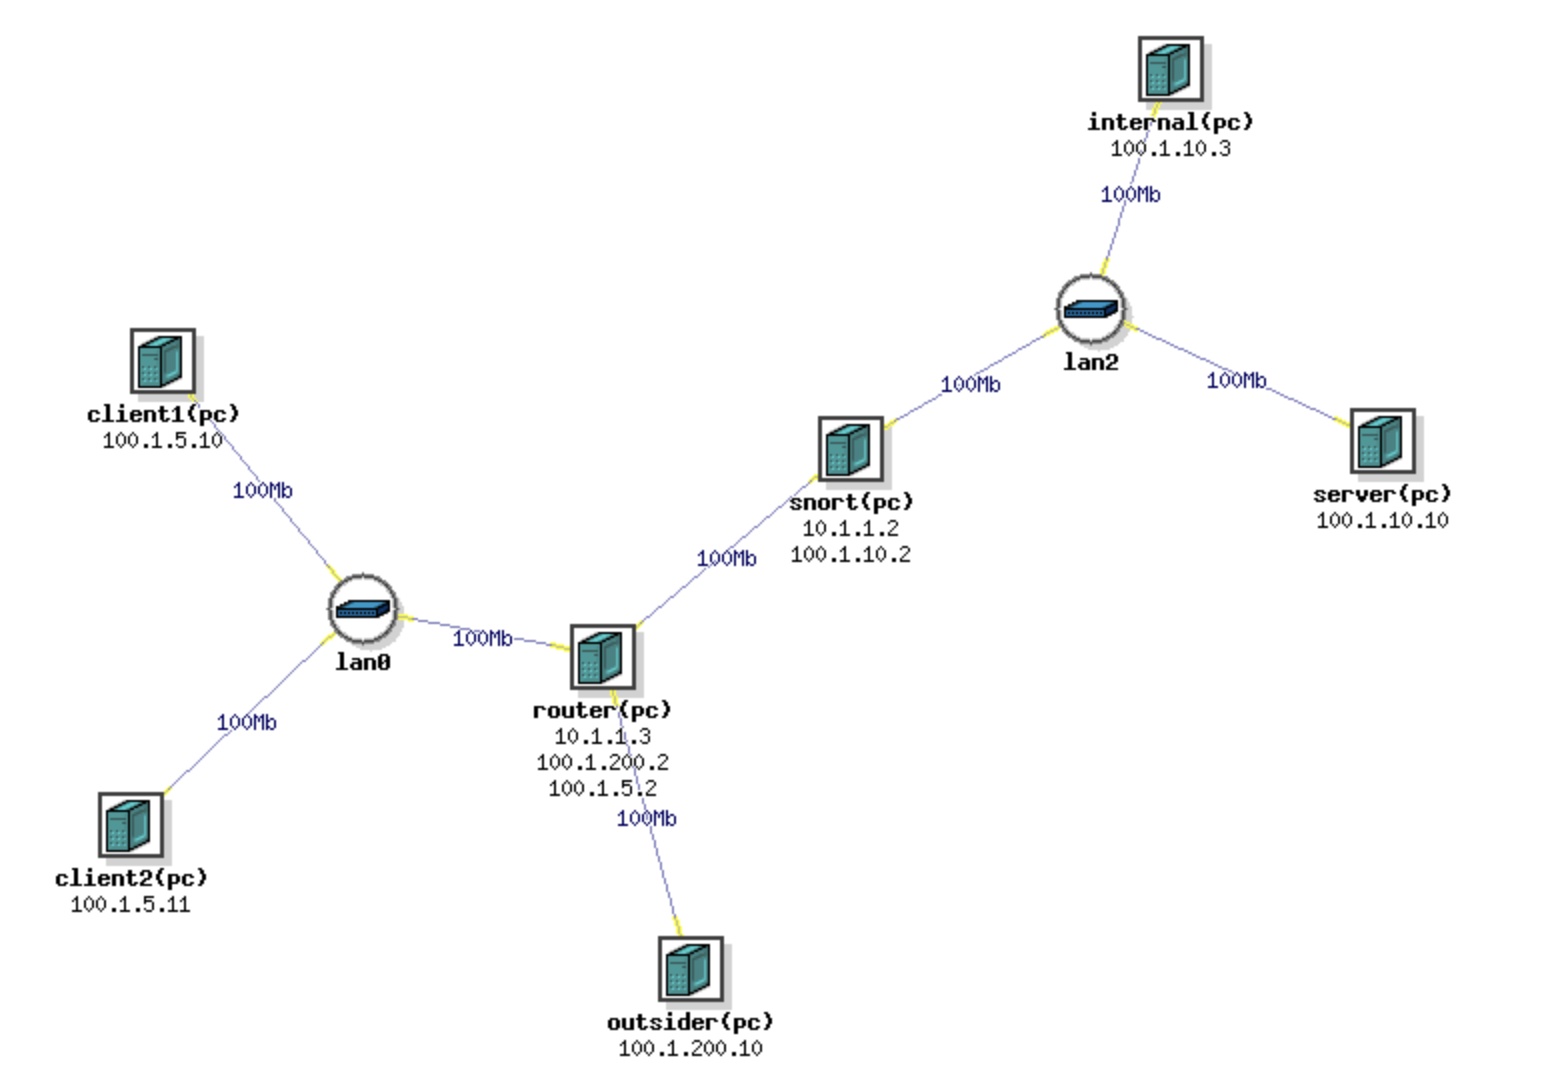
\includegraphics[width=\textwidth]{../drawable/network.png}
    \caption{Network setup for the exercise.}
\end{figure}

\clearpage
\newpage

\subsection{Basic exercises}

\subsubsection{Start Snort Without rules}

Connect to \verb=users.deterlab.net=. SSH into the \verb=snort= experiment node.

Start snort without any rules by entering the command \verb=sudo snort --daq nfq -Q -v=. You should see a large number of packets being reported by Snort.

Open another terminal and SSH again into \verb=users.deterlab.net= and the \verb=snort= node. In this terminal run \verb=tcpdump= to capture the data going to and from the \verb=client1=. This should be on the interface with an IP Address in the \verb=10.1.1.0/24= range. 

You can run tcpdump using the command:

\begin{code}{Code for using tcpdump}
**# tcpdump -i [interface] -s 0 -w /tmp/dump.pcap**
\end{code}
    
Allow this to run for 30 seconds and then tcpdump by pressing \verb=^C=. Let the Snort process continue running. Now run

\begin{code}{Processing the obtained data.}
**# /share/education/SecuringLegacySystems_JHU/process.pl /tmp/dump.pcap**
\end{code}

This will produce a set of $x,y$ coordinates where $x$ is time and $y$ is number of packets in that second.

\begin{theorem}
    Respond to the following points. 
    \begin{enumerate}
        \item What happens to the traffic to client1 when Snort is not running?
        \item Is this a good thing?
        \item Based on Snort's output what can you say about the application? What port does it connect to?
        \item Please attach a graph of the traffic over time to your answers
        \item What does the "-Q" option do in Snort?
        \item What does the "--daq nfq" option do in Snort?    
    \end{enumerate}
\end{theorem}

\begin{proof}
    These are the answers.
    \begin{enumerate}
        \item When snort is not running, all traffic gets dropped.
        \item Not really. We can see that there are \verb=client2= and \verb=outsider= that are continuosly sending traffic to \verb=server=, but it also gets dropped when snort is not running. Since Snort is woking in inline mode, all traffic is supposed to pass through the snort bridge.
        \item The application accepts incoming connections on port \verb=7777=.
        \item See the graph at the end of the numbered section.
        \item The -Q option tells snort to process packets in inline mode.
        \item The --daq nfq option tells snort to use the \verb=nfq= DAQ module.
    \end{enumerate}

    \begin{figure}[h!]
        \centering
        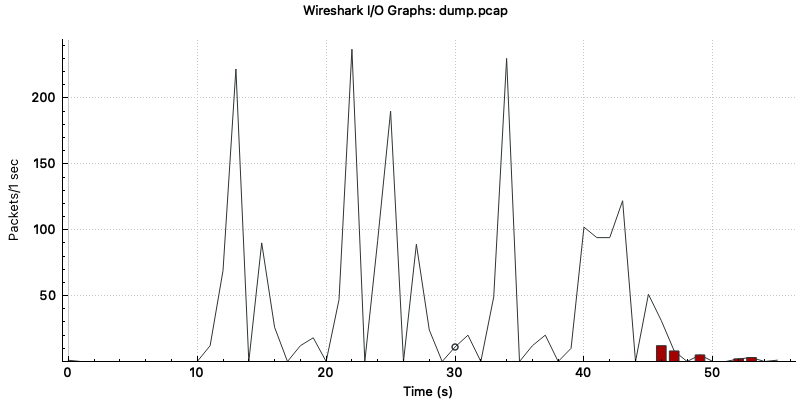
\includegraphics[width=\textwidth]{../drawable/traffic.png}
        \caption{Traffic over time.}
    \end{figure}

\end{proof}

\subsubsection{Analyze Network Traffic}

Connect to the \verb=router= node. Use \verb=ifconfig= to determine which network interfaces connect to which network. Run \verb=tcpdump= to capture the data going to the server. This should be on the interface with an IP Address in the \verb=10.0.1.0/24= range. 

You can run tcpdump with the same command as in Part 1. Let this run for around a minute before terminating it by pressing \verb=^C=. Copy this data to your computer via SCP and open it using Wireshark. 

\begin{theorem}
    The request that the client sends the server is broken into four parts. What are these parts and what order does they appear in? How are these parts seperated in the request?
    Is this is a secure way for the client to send requests to the server? Explain your answer.
    Can you recover one of the files sent by the server to a client? If so attach the file, a pcap the relevant packets and indicate which client this was sent to.
\end{theorem}

\begin{proof}
\end{proof}

\subsubsection{Write Rules to Guard Against Simple Requests}

In that terminal where snort is running stop it with \verb=^C=. Write a configuration file for snort using the command, named \verb=snort.config=. Add the following snort rule that prevents .xml files from being sent out.

\begin{code}{Code to add to the config.}
reject tcp 100.1.0.0/16 ANY -> 100.1.10.10 [Port from Question 3]
    (msg: "XML Read Attempt Detected"; sid:1; content:".xml";)
\end{code}

Using this rule as an example write a rule that prevents classified data from being sent to the outsider computer, but does not prevent it from being sent to any other computers. Now you must make a directory for snort alerts, called \verb=alerts=. Start snort using your new rule with the command:

\begin{code}{Code to start snort.}
**# snort --daq nfq -Q -c snort.config -l alerts**
\end{code}

Log onto \verb=client1=, \verb=client2= and \verb=outsider= to see if these rules worked. If you aren't sure go to the folder \verb=/home/test= and delete the existing .txt and .xml files then see which ones are recreated. You can also run the program FileClient manually to find out.
Questions:

\begin{theorem}
    Respond to the following points.
    \begin{itemize}
        \item What rule did you use to secure the "classified" file?
        \item Capture and compare the network traffic for the serverwhen filtering these results using your configuration file and when no file is used. Attach the graph showing packet rate over time for both of these cases to your submission.
        \item Can you think of any others files or extensions that should be filtered against?
    \end{itemize}
\end{theorem}

\clearpage
\newpage

\subsection{Intermediate tasks}
\subsubsection{DOS defense}

Make sure you have your filtering rule engaged on Snort. Using the \verb=flooder= tool on client1 create a packet flood attack against the server from. Set a high rate of 100,000 requests and duration of 100 seconds. Just typing flooder on command line should give you a list of options you can use.

Create a new Snort configuration that also includes a rate filter rule. These follow the following format:

\begin{code}{Format for rate filters.}
rate_filter gen_id 1, sig_id [sid of event], 
track [by_src, by_dst or by_rule], count [number of events], 
seconds [number of seconds], new_action drop, 
timeout [number of seconds]
\end{code}

You may need to write a new rule for the rate filter to apply to. 

Create an event filter for your rate filter. These follow the format:

\begin{code}{Format for event filters.}
event_filter gen_id 1, sig_id [sid_number], 
track [by_src, by_dst or by_rule], count [number of events],
seconds [number of seconds],
type [limit, threshold or both]
\end{code}

\begin{theorem}
    Respond to the following points.
    \begin{enumerate}
        \item Collect the traffic at the server and the router when there is and is not an attack with rules in place that only guard against the attacks metioned in the basic exercises. Create a graph of this traffic over time.
        \item Repeat the previous step but now with the rate filtering rules enabled.
        \item For a DOS attack should rate filtering rules be paired with event filtering rules?
        \item Try changing the new action in the rate filter to "reject" instead of "drop". What does this do to the traffic and why do you think this is? Is this a good or a bad thing?
        \item Check which interface Snort connects to the router to using ifconfig. Once you have this information try the above test against while specifying that interface instead of using the default value. This argument will look something like --daq-var device=eth1. Did this change your results. If so attach a graph and explain the change occured.
        \item Are there any changes you can make outside of Snort to help guard against this attack? If so what are they?
        \item Try running the FileClient program from client2 while this attack is underway. What happens when you have the various rulesets configured?
    \end{enumerate}
\end{theorem}


\subsubsection{Secure Traffic on the Network}

Make sure that Snort is running with all your filtering rules in place. Now, review the pcap data you gathered while analyzing network traffic on the router.

Review the network topology on DETER. Notice that the internal computer is able to bypass Snort entirely!

Verify this by logging onto the internal computer and checking the folder \verb=/home/test=. You should see that it is able to freely download files that your rules do not permit.

Replace the direct route to the server using the following command:

\begin{code}{Code for replacing the direct route to the server.}
**# route add -host server gw snort**
\end{code}

This should cause traffic to the server to be routed through Snort. Perform a trace route to verify this with the command \verb=traceroute server=.

\begin{theorem}
    Respond to the following points.
    \begin{enumerate}
        \item Based on the traffic you analyzed what changes could be made to the network to enhance the security of communications coming from client1, client2 and outsider?
        \item What software packages would this require and where should these be installed? Would this cause problems for Snort?
        \item How should the server be configured to prevent internal attacks?
        \item Would this require you to change your Snort configuration in any way?
    \end{enumerate}
\end{theorem}

\clearpage
\newpage

\subsection{Advanced Tasks}
\subsubsection{Code Execution Vulnerability}

A vulnerability was found with the FileServer that causes it to execute the contents of the filename field if certain conditions are met.

To do this point, you must download the file \verb=/home/test/FileServer.jar= from the server. Analyze the file using a Java decompiler such as JD-GUI to find the vulnerability.

\begin{theorem}
    Respond to the following points.
    \begin{enumerate}
        \item What are the conditions required for this attack to take place?
        \item Create a Snort rule to defend against this attack. You may want to be use pcre instead of content for this rule.
        \item What effect does this rule have on legitimate traffic?
    \end{enumerate}
\end{theorem}

\subsubsection{Defend Against ASCII Encoding}

An additional "feature" was recently brought to the attention of the security team: the application has a limited ability to before ASCII decoding. This decoding is triggered whenever the server encounters a \% followed by a number between 0 and 255 at which point the sequence is converted to a single ASCII character.

Now go to the following directory: 
\begin{verbatim}
    /usr/local/snort-2.9.2.2/src/dynamic-examples/dynamic-preprocessor
\end{verbatim}

This contains an example Snort preprocessor. Snort preprocessors allow for advanced data manipulation to normalize data and perform other functions that normal rules cannot. All Snort preprocessors are coded in C.

Open up \verb=spp_example.c= and take a look at the structure. The main function of interest to you in this case is \verb=ExampleProcess= which is used to process packet data before other rules have a chance to access it. Copy the include folder using the following command:

\begin{code}{Code for including the folder.}
**# cp /usr/local/snort-2.9.2.2/src/dynamic-preprocessors/include/ ..**
\end{code}

You should now be able to compile and install this preprocessor using the command:

\begin{code}{Make command.}
**# make && make install**
\end{code}

Once this has been installed you can use this preprocessor in Snort. To do this edit your configuration file by adding the following lines at the top of the file which tell Snort to auto-generate the decoder rules so you don't have to, the location of the preprocessor library and the preprocessor you wish to use along with all of its arguments (in this case just the port to use):

\begin{code}{Code for adding the preprocessor to the configuration file.}
config autogenerate_preprocessor_decoder_rules
dynamicpreprocessor directory /usr/local/lib/snort_dynamicpreprocessor/
preprocessor dynamic_example: port [Port from Question 3]
\end{code}

Once you have made these changes try to run Snort using your configuration file. At this point it should behave exactly as before, but it now has a preprocessor loaded which you can edit to meet your needs as an ASCII decoder.

\begin{theorem}
    Respond to the following points.
    \begin{enumerate}
        \item Were you able to bypass your existing rules because of this feature? If so what input strings did you use?
        \item Can you think of a content rule to effectively defend against an attack that uses this feature? Would this affect legitimate traffic?
        \item Snort includes support for user written preprocessors that can render data for Snort's other rules. How would the use of a preprocessor help with this task?
        \item Write a preprocessor to help with this task. Please attach all of the functions you used and the snort.config file that called the preprocessor.
    \end{enumerate}
\end{theorem}

\endgroup
\end{document}